\documentclass[12pt,oneside]{article}

%%%%%%%%%%%%%%%%%%%%%%%%%%%%
%%   Zusaetzliche Pakete  %%
%%%%%%%%%%%%%%%%%%%%%%%%%%%%
\usepackage{acronym}
\usepackage{enumerate}  
\usepackage{a4wide}
\usepackage{fancyhdr}
\usepackage{graphicx}
\usepackage{palatino}
\usepackage{blindtext}
\usepackage{multirow}
\usepackage[ruled,longend]{algorithm2e}
\usepackage{float}


%folgende Zeile auskommentieren für englische Arbeiten
\usepackage[ngerman]{babel}

\usepackage[T1]{fontenc}
\usepackage[utf8]{inputenc}
\usepackage[bookmarks]{hyperref}
\usepackage[justification=centering]{caption}
\usepackage[style=chicago-authordate,natbib=true,backend=biber]{biblatex}
\usepackage{csquotes}
\bibliography{literatur}

\renewcommand{\baselinestretch}{1.5} 
%%%%%%%%%%%%%%%%%%%%%%%%%%%%%%
%% Definition der Kopfzeile %%
%%%%%%%%%%%%%%%%%%%%%%%%%%%%%%

\pagestyle{fancy}
\fancyhf{}
\cfoot{\thepage}
\setlength{\headheight}{16pt}

%%%%%%%%%%%%%%%%%%%%%%%%%%%%%%%%%%%%%%%%%%%%%%%%%%%%%
%%  Definition des Deckblattes und der Titelseite  %%
%%%%%%%%%%%%%%%%%%%%%%%%%%%%%%%%%%%%%%%%%%%%%%%%%%%%%

\newcommand{\JMUTitle}[9]{

  \thispagestyle{empty}
  \vspace*{\stretch{1}}
  {\parindent0cm
  \rule{\linewidth}{.7ex}}
  \begin{flushright}
    \vspace*{\stretch{1}}
    \sffamily\bfseries\Huge
    #1\\
    \vspace*{\stretch{1}}
    \sffamily\bfseries\large
    #2
    \vspace*{\stretch{1}}
  \end{flushright}
  \rule{\linewidth}{.7ex}

  \vspace*{\stretch{1}}
  \begin{center}
    
\includegraphics[width=3in]{logo} \\
    \vspace*{\stretch{1}}
    \Large Hausarbeit  \\

    \vspace*{\stretch{2}}
   \large Autor: Hannes Frey \\
    \vspace*{\stretch{1}}
    \large Betreuer:  Roland Kiefer \\[1mm]
    
    \vspace*{\stretch{1}}
    \large Stuttgart, den #6
  \end{center}
}


%%%%%%%%%%%%%%%%%%%%%%%%%%%%
%%  Beginn des Dokuments  %%
%%%%%%%%%%%%%%%%%%%%%%%%%%%%

\begin{document}

  \JMUTitle
      {Kryptowährungen }        % Titel der Arbeit
      {Funktionsweise und Ausblick}                        % Vor- und Nachname des Autors
      
      {Wirtschaftswissenschaftlichen Fakultät}  % Name der Fakultaet
      {W"urzburg 2018}                          % Ort und Jahr der Erstellung
      {31.05.2021}                              % Tag der Abgabe
      {Prof. Dr. Christian Janiesch}               % Name des Erstgutachters
      {Zweitgutachter}                          % Name des Zweitgutachters
      {Pr"ufungsdatum}                          % Datum der muendlichen Pruefung

  \clearpage

\lhead{}
\pagenumbering{Roman} 
    \setcounter{page}{1}

\tableofcontents
\clearpage

\addcontentsline{toc}{section}{\listfigurename}
\listoffigures

\addcontentsline{toc}{section}{\listtablename}
\listoftables
\clearpage

%%%%%%%%%%%%%%%%%%%%%%%%%%%%
%%  Kurzzusammenfassung   %%
%%%%%%%%%%%%%%%%%%%%%%%%%%%%
\markboth{Zusammenfassung}{Zusammenfassung}
\section*{Zusammenfassung}
\blindtext
\clearpage

%%%%%%%%%%%%%%%%%%%%%%%%%%%%
%%  Abstract   %%
%%%%%%%%%%%%%%%%%%%%%%%%%%%%
%\markboth{Abstract}{Abstract}
%\section*{Abstract}
%\blindtext



%%%%%%%%%%%%%%%%%%%%%%%%%%%%
%%  Einstellungen  %%
%%%%%%%%%%%%%%%%%%%%%%%%%%%%
\cleardoublepage
\pagenumbering{arabic}  
    \setcounter{page}{1}
\lhead{\nouppercase{\leftmark}}

%%%%%%%%%%%%%%%%%%%%%%%%%%%%
%%  Hauptteil  %%
%%%%%%%%%%%%%%%%%%%%%%%%%%%%

\section{Einleitung} \label{einleitung}

Seit der Erfindung des Internets in den 90er Jahren befindet sich die Welt im digitalen Wandel. Das World Wide Web bietet Funktionen, die vor 20 Jahren als unvorstellbar galten, und das enorme Wachstumspotential der Technik ist noch lange nicht ausgeschöpft. Im Jahre 2009 ist diesem Zweig auch eine digitale Währung entsprungen und diese begleitet uns seither: Die Bitcoin. 
Doch bei dieser einen Währung ist es nicht geblieben, denn in den vergangenen Zwölf Jahren haben sich tausende weitere dazu gesellt und eine eigene Ökonomie erschaffen, die das Potenzial einer digitalen Revolution besitzt.
Kryptowährungen haben es dabei zuletzt wieder vermehrt in die Abendnachrichten geschafft, sei es wegen neuer Allzeithochs oder Kursabstürzen. 

\begin{figure}[h]
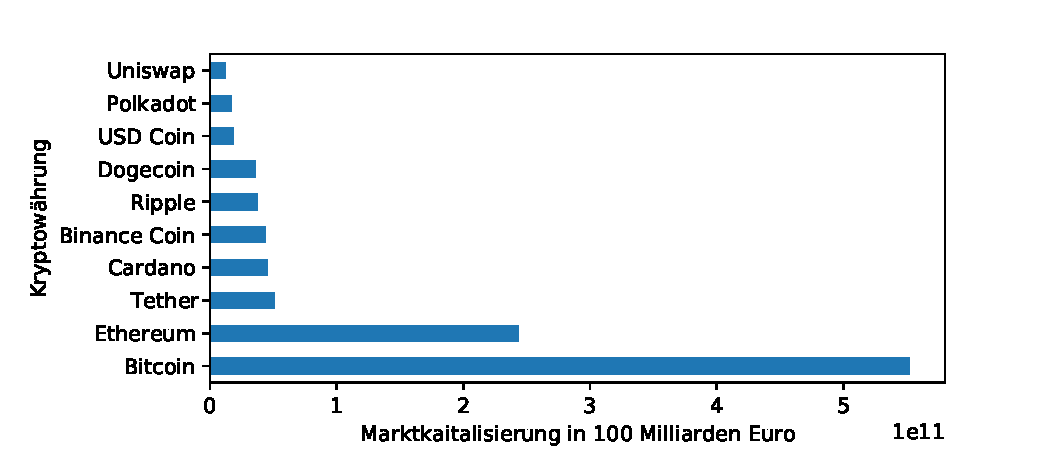
\includegraphics[scale=0.9]{./images/marketcap.pdf}
\caption{Marktkapitalisierung der Zehn größten Krytowährungen in Euro}
\centering
\end{figure}


In der folgenden Arbeit werden Funktionsweise, Chancen und Risiken sowie die wirtschaftliche Bedeutung von Kryptowährungen genauer behandelt.

\subsection{Bitcoin}
\subsection{Altcoins und Forks}
\subsection{Ethereum und Smart Contracts}

\section{Chancen und Risiken}


\section{Konsequenzen}

\subsection{Heutiges Geldsystem}

%%%%%%%%%%%%%%%%%%%%%%%%%%%%
%% Literaturverzeichnis wird 
%% automatisch eingefügt
%%%%%%%%%%%%%%%%%%%%%%%%%%%%
\clearpage
\lhead{}
\printbibliography
\addcontentsline{toc}{section}{\bibname}


%%%%%%%%%%%%%%%%%%%%%%%%%%%%
%% Eidesstattliche Erklärung
%% muss angepasst werden 
%% in Erklaerung.tex
%%%%%%%%%%%%%%%%%%%%%%%%%%%%
\newpage
\begin{otherlanguage}{ngerman}
\thispagestyle{empty}
\section*{Eidesstattliche Erklärung}
\thispagestyle{empty}
Hiermit versichere ich, die vorliegende Arbeit selbstständig verfasst und keine anderen als die angegebenen Quellen und Hilfsmittel benutzt sowie die Zitate deutlich kenntlich gemacht zu haben.
\newline
Ich erkläre weiterhin, dass die vorliegende Arbeit in gleicher oder ähnlicher Form noch nicht im Rahmen eines
anderen Prüfungsverfahrens eingereicht wurde.
\vspace{4\baselineskip}\\
Stuttgart, den \today \hfill
 \includegraphics[width=0.3\textwidth]{./images/unterschrift.png}
\vspace{4\baselineskip}\\
\end{otherlanguage}

\end{document}
